% SPDX-License-Identifier: Apache-2.0
%
% A network on chip in TxHDL. Built by //docs:noc. Every listing is
% included from the tree.
\documentclass[journal,9pt]{IEEEtran}

\newcommand{\listingsize}{\fontsize{6}{7}\selectfont}
% SPDX-License-Identifier: Apache-2.0
%
% The house preamble, shared by every document in this directory. Loaded
% after \documentclass, before \title. Keeping it in one file is what
% stops two articles drifting apart in font, listing style or figure
% style.
% Computer Modern. IEEEtran selects Times (ptm) by default, so the face has
% to be chosen explicitly.
%
% Latin Modern is the Computer Modern variety used here, and the choice is
% forced rather than aesthetic. Under T1 encoding, plain `cmr` has no Type 1
% outlines unless cm-super is installed, and it is not in the pinned
% distribution, so pdflatex falls back to EC bitmaps and every glyph in the
% PDF becomes a Type 3 font. That was measured: the first build produced a
% document with 10 Type 3 fonts and no Type 1. Latin Modern is Computer
% Modern redrawn with a full T1 repertoire and real .pfb outlines, so the
% same design comes out scalable.
\usepackage[T1]{fontenc}
\usepackage[utf8]{inputenc}
\usepackage{lmodern}
% microtype is not in the pinned TeX distribution. emergencystretch alone
% keeps the two-column measure from producing overfull lines.
\setlength{\emergencystretch}{3em}

\usepackage{amsmath}
\usepackage{amssymb}
\usepackage{amsthm}
\usepackage{booktabs}
\usepackage{array}
% enumitem is not in the pinned TeX distribution; the list spacing below
% does what \setlist would have done.
\usepackage{float}
\usepackage{xcolor}
\usepackage{listings}
\usepackage{tikz}
\usetikzlibrary{arrows.meta,positioning,fit,backgrounds,calc}
\usepackage[hidelinks,bookmarks=true]{hyperref}

% Numbered, definition-style box for a rule the reader is meant to apply.
\theoremstyle{definition}
\newtheorem{rulebox}{Rule}
\newtheorem{example}{Example}

% Unnumbered asides.
\theoremstyle{remark}
\newtheorem*{tip}{Tip}
\newtheorem*{pitfall}{Pitfall}

% Tighter lists, in place of enumitem's \setlist.
\setlength{\topsep}{2pt}
\setlength{\itemsep}{1pt}
\setlength{\parsep}{0pt}

\newcommand{\code}[1]{\texttt{#1}}
\newcommand{\term}[1]{\emph{#1}}

% Syntax highlighting. Four roles, distinguishable in colour and still
% distinguishable in greyscale, because an IEEE article gets printed: the
% keyword is the only bold role, the comment is the only italic one, and the
% two remaining roles differ in lightness as well as in hue.
\definecolor{kwblue}{RGB}{20,60,150}
\definecolor{cmtgreen}{RGB}{90,120,90}
\definecolor{strred}{RGB}{150,50,40}
\definecolor{numgray}{gray}{0.45}
\definecolor{framegray}{gray}{0.70}
\definecolor{bgshade}{gray}{0.97}
% A darker fill for figure cells. The listing background has to stay very
% light to keep code readable; a figure cell has to be clearly shaded or the
% distinction it draws is invisible in print.
\definecolor{cellshade}{gray}{0.90}

% The listing size is the document's choice, because it depends on the
% column: a two-column article sets `\listingsize` to 6pt and keeps its
% listings within 70 columns, a one-column document keeps the body size
% and includes source files at 80. Lines are never broken; a line that does not fit
% overflows the frame, which is visible, rather than wrapping, which is
% not.
\providecommand{\listingsize}{\scriptsize}

% `'` is deliberately not a string delimiter: the language uses it for loop
% labels, as Rust does, so treating it as a quote would swallow the rest of
% the line.
\lstdefinestyle{txhdl}{
  basicstyle=\ttfamily\listingsize,
  keywordstyle=\bfseries\color{kwblue},
  commentstyle=\itshape\color{cmtgreen},
  stringstyle=\color{strred},
  numberstyle=\tiny\color{numgray},
  morekeywords={mod,use,pub,const,type,struct,enum,trait,impl,fn,async,let,mut,
    match,if,else,loop,while,for,in,break,continue,return,as,await,
    module,bus,channel,transaction,protocol,pipeline,flow,seq,config,
    port,stage,pipe,instance,connect,bind,tag,domain,blackbox,foreign,
    property,role,signal,handler,true,false,
    sequence,interface,modport,implements,package,import,var,wire,func,proc,
    case,default,next,fork,branch,join,state,fsm},
  morecomment=[l]{//},
  morestring=[b]",
  showstringspaces=false,
  columns=fullflexible,
  keepspaces=true,
  breaklines=false,
  % Framed, so a listing is bounded rather than floating in the column.
  frame=single,
  rulecolor=\color{framegray},
  framesep=3pt,
  backgroundcolor=\color{bgshade},
  xleftmargin=3pt,
  xrightmargin=3pt,
  aboveskip=6pt,
  belowskip=6pt,
  % Every listing is numbered and captioned, so it can be referred to by
  % number. `caption` without `float` numbers the listing and leaves it
  % where it was written, which is what a listing in running prose needs.
  captionpos=b,
  abovecaptionskip=2pt,
  belowcaptionskip=6pt,
}

% Figures drawn as text. Framed the same way, and with the highlighting
% switched off, because a box-and-arrow diagram is not code and half its
% words turning blue reads as an accident. Setting a style adds keys rather
% than clearing the ones already set, so the three roles are neutralised by
% hand rather than by leaving them out.
\lstdefinestyle{ascii}{
  basicstyle=\ttfamily\listingsize,
  keywordstyle=\ttfamily,
  commentstyle=\ttfamily,
  stringstyle=\ttfamily,
  columns=fullflexible,
  keepspaces=true,
  frame=single,
  rulecolor=\color{framegray},
  framesep=3pt,
  backgroundcolor=\color{bgshade},
  xleftmargin=3pt,
  xrightmargin=3pt,
  aboveskip=6pt,
  belowskip=6pt,
}
\lstset{style=txhdl}

% House TikZ styles. `shorten` lives on the arrow styles rather than on each
% arrow, so every arrow in the document gets the gap, including ones added
% later. TikZ clips a path at a node's border, so without it an arrowhead
% butts against the box with no gap at all. Keep `node distance` well above
% twice the shorten, or the arrow shrinks to nothing.
\tikzset{
  box/.style={draw,rounded corners=2pt,align=center,inner sep=4pt,
              font=\footnotesize},
  boxf/.style={box,fill=bgshade},
  lbl/.style={font=\scriptsize\itshape,align=center},
  fl/.style={-{Stealth[length=4pt]},shorten >=2.5pt,shorten <=2.5pt},
  fld/.style={fl,dashed},
}



\InputIfFileExists{buildstamp.tex}{}{}
\providecommand{\buildstamp}{Draft build (outside the Bazel flow).}

% A range of a source file of the network, by its begin/end markers.
\newcommand{\nocpart}[4]{%
\lstinputlisting[rangebeginprefix=//\ begin\{,rangebeginsuffix=\},%
rangeendprefix=//\ end\{,rangeendsuffix=\},includerangemarker=false,%
linerange=#2-#2,caption={#3},label={#4}]{lib/parts/src/bus/noc/#1}}

\title{A Network on Chip in TxHDL}

\author{Filip Filmar and Dragiša Janković%
\thanks{Both authors are independent. Filip Filmar is the
corresponding author, at f@hdlfactory.com; Dragiša Janković is
reached at linkedin.com/in/dragisa-jankovic.}%
\thanks{This is the tutorial on the network, for a reader who knows
the AXI link~\cite{axi} and wants more than one host and more than
one peripheral on it. Every listing is included from the project
repository \code{HDL/txhdl} at build time. The cover~\cite{cover}
lists every document.}%
\thanks{The authors used a large language model, Claude, as an
assistant in exploring the concepts and in writing and constructing
the documents and the programs; every commit of the repository says
so and carries the prompts that led to it, verbatim.}%
\thanks{\buildstamp}}

\markboth{A Network on Chip in TxHDL}{Filmar and Janković: A Network on Chip in TxHDL}

\begin{document}
\maketitle

\begin{abstract}
A router puts several peripherals behind one host. A network puts
several of both on a lattice and lets any of them reach any other. The
network here is nodes with a two-way link to each of their four
neighbours and a fifth, the exit, where something that is not a node
attaches; every link is two virtual channels; routing is dimension
order; and the exit is a bridge with AXI on one side and packets on
the other. Neither end knows the network is there: a host issues a
burst and awaits its answer as it would on a link, and a peripheral
accepts a transaction and answers it as it would.
\end{abstract}


\begin{figure}[htbp]
\centering
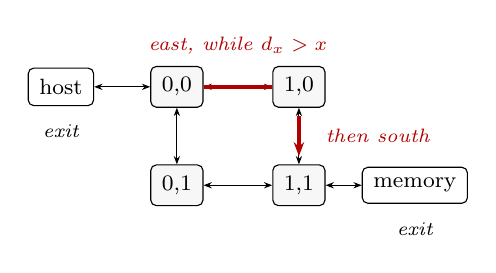
\begin{tikzpicture}[x=1.55cm, y=-1.25cm, font=\scriptsize]
  \node[boxf] (n00) at (0,0) {0,0};
  \node[boxf] (n10) at (1,0) {1,0};
  \node[boxf] (n01) at (0,1) {0,1};
  \node[boxf] (n11) at (1,1) {1,1};
  \draw[{Stealth[length=3pt]}-{Stealth[length=3pt]}] (n00) -- (n10);
  \draw[{Stealth[length=3pt]}-{Stealth[length=3pt]}] (n01) -- (n11);
  \draw[{Stealth[length=3pt]}-{Stealth[length=3pt]}] (n00) -- (n01);
  \draw[{Stealth[length=3pt]}-{Stealth[length=3pt]}] (n10) -- (n11);
  \node[box] (h) at (-0.95,0) {host};
  \node[box] (m) at (1.95,1) {memory};
  \draw[{Stealth[length=3pt]}-{Stealth[length=3pt]}] (h) -- (n00);
  \draw[{Stealth[length=3pt]}-{Stealth[length=3pt]}] (n11) -- (m);
  \draw[-{Stealth[length=5pt]}, very thick, red!70!black, shorten >=3pt,
        shorten <=3pt]
       (n00) -- (n10) -- (n11);
  \node[lbl, red!70!black] at (0.5,-0.42) {east, while $d_x > x$};
  \node[lbl, red!70!black, anchor=west] at (1.14,0.5) {then south};
  \node[lbl] at (-0.95,0.45) {exit};
  \node[lbl] at (1.95,1.45) {exit};
\end{tikzpicture}
\caption{A two by two lattice, and the way a burst takes from the host
at 0,0 to the memory at 1,1. Dimension order: X first and then Y, so a
packet never turns from Y back into X and no cycle of waiting can form
among the links.}
\label{fig:n-lattice}
\end{figure}

\section{What a Link Carries}
\label{sec:n-pkt}

Figure~\ref{fig:n-lattice} is the shape of it. A link carries one beat
of one AXI channel, addressed to a node and stamped with the
node it came from.

\nocpart{pkt.rs}{pkt}{A packet.}{lst:n-pkt}

It is one shape, as wide as the widest beat needs, for the same reason
the GPU's instruction is~\cite{gpu}: every field a step reads has to
be at a fixed place, and a link that carried a header and then a body
would want a sequencer at both ends before anything else worked. A
read address beat leaves the data and the strobe at zero; a write
response leaves the address at zero; \code{Chan} says which fields
mean anything.

The source is carried rather than remembered. A node keeps no table of
who asked, and an answer finds its way home by reading the stamp the
question arrived with.

\section{Virtual Channels}
\label{sec:n-vc}

There are two, one for requests and one for responses, and they share
nothing: a node is a switch per virtual channel, and each switch has
its own buffers.

That is not tidiness, it is the thing that keeps the network from
seizing. A peripheral answers a request by sending a response. If a
full path of requests could hold up the responses behind it, the
responses that would empty that path could never leave, and the
network would stop with every buffer full and nothing able to move. On
two channels the response has a way through whatever the requests are
doing.

\section{A Node}
\label{sec:n-node}

Routing is dimension order: a packet goes east or west until it is in
its destination's column, then north or south until it is at its node,
then out of the exit.


\begin{figure}[htbp]
\centering
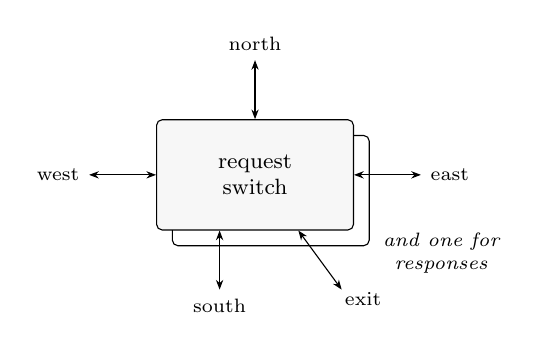
\begin{tikzpicture}[x=1cm, y=1cm, font=\scriptsize]
  % The response switch, behind: a node has two of these and they
  % share nothing.
  \node[box, fill=white, minimum width=2.5cm, minimum height=1.4cm]
       (p) at (0.2,-0.2) {};
  \node[lbl, anchor=north west] at (1.5,-0.62) {and one for\\responses};
  \node[boxf, minimum width=2.5cm, minimum height=1.4cm] (q) at (0,0)
       {request\\switch};
  % Each link leaves the side it is named for.
  \draw[{Stealth[length=3.5pt]}-{Stealth[length=3.5pt]}]
       (q.north) -- ++(0,0.75) node[above, font=\scriptsize] {north};
  \draw[{Stealth[length=3.5pt]}-{Stealth[length=3.5pt]}]
       ($(q.south)+(-0.45,0)$) -- ++(0,-0.75)
       node[below, font=\scriptsize] {south};
  \draw[{Stealth[length=3.5pt]}-{Stealth[length=3.5pt]}]
       (q.west) -- ++(-0.85,0) node[left, font=\scriptsize] {west};
  \draw[{Stealth[length=3.5pt]}-{Stealth[length=3.5pt]}]
       (q.east) -- ++(0.85,0) node[right, font=\scriptsize] {east};
  % The fifth port: where something that is not a node attaches.
  \draw[{Stealth[length=3.5pt]}-{Stealth[length=3.5pt]}]
       ($(q.south)+(0.55,0)$) -- ++(0.55,-0.75)
       node[below right, font=\scriptsize, inner sep=1pt] {exit};
\end{tikzpicture}
\caption{A switch: a two-way link on each of the four sides it is
named for, and a fifth port, the exit, where something that is not a
node attaches. A node is two of these, one per virtual channel, and
they share nothing, so a request held up behind a full buffer cannot
hold up the response that would empty it. A host's bridge puts
requests into the one and takes responses out of the other; a
peripheral's bridge does the reverse.}
\label{fig:n-node}
\end{figure}

\nocpart{switch.rs}{route}{The whole of the routing.}{lst:n-route}

On a lattice that is deadlock free with nothing else said, because a
packet never turns from Y back into X, so no cycle of waiting can
form among the links.

One packet moves through a switch per cycle. Each input's direction
and the room at the port it wants are worked out first, so that an
input whose port is full does not hold up the others, and the choice
among those that can move is by a fixed order that serves the four
links before the exit: a node does not starve the network in order to
feed itself. A fair arbiter would be the next thing to write; the
order here is a fixed priority and this document would rather say so
than not.

\nocpart{switch.rs}{run}{The switch, a cycle at a
time.}{lst:n-switch}

\nocpart{node.rs}{run}{A node: a switch per virtual channel. The
twenty ports are written out one by one because a lowered unit's
ports are a positional tuple and a named type for a side is
refused.}{lst:n-node}

\section{The Exit}
\label{sec:n-bridge}

A bridge, AXI on one side and packets on the other, in two halves.

\begin{figure}[htbp]
\centering
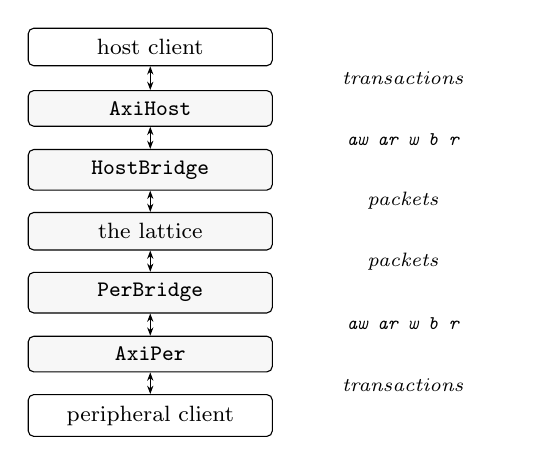
\begin{tikzpicture}[x=1cm, y=-0.78cm, font=\scriptsize,
                    every node/.style={minimum width=3.1cm}]
  \node[box] (hc) at (0,0) {host client};
  \node[boxf] (ht) at (0,1) {\code{AxiHost}};
  \node[boxf] (hb) at (0,2) {\code{HostBridge}};
  \node[boxf] (nw) at (0,3) {the lattice};
  \node[boxf] (pb) at (0,4) {\code{PerBridge}};
  \node[boxf] (pt) at (0,5) {\code{AxiPer}};
  \node[box] (pc) at (0,6) {peripheral client};
  \foreach \a/\b in {hc/ht,ht/hb,hb/nw,nw/pb,pb/pt,pt/pc}
    \draw[{Stealth[length=3pt]}-{Stealth[length=3pt]}] (\a) -- (\b);
  \node[lbl, anchor=west] at (1.65,0.5) {transactions};
  \node[lbl, anchor=west] at (1.65,1.5) {\code{aw ar w b r}};
  \node[lbl, anchor=west] at (1.65,2.5) {packets};
  \node[lbl, anchor=west] at (1.65,3.5) {packets};
  \node[lbl, anchor=west] at (1.65,4.5) {\code{aw ar w b r}};
  \node[lbl, anchor=west] at (1.65,5.5) {transactions};
\end{tikzpicture}
\caption{What is between the two clients. Neither end knows the
network is there: the host issues a burst and awaits its answer as it
would on a link, and the peripheral accepts a transaction and answers
it as it would.}
\label{fig:n-layers}
\end{figure}


The host half packs an address phase into a packet addressed by a map
of three ranges, whose last entry is the default route: give it a mask
of zero and every address that matched nothing else goes there. A
design that states its map that way has no address the network does
not know, which is why neither half has to answer for one.

A write of one beat is one packet, carrying its address phase and its
data together. That is what the hosts in this tree make, and it is
what keeps two of them from interleaving their write data at a
peripheral that has one port: AXI4 puts no identifier on the write
data channel, so a beat that arrived between another host's address
phase and its beat could not be told apart. A burst of more than one
beat wants a virtual channel per source, or reassembly at the
peripheral, and this bridge carries none.

\nocpart{bridge.rs}{hostrun}{The host half.}{lst:n-host}

The peripheral half unpacks a request into the channels a
peripheral's tracker reads, and packs the answers back to the node
the request came from.

It also renames. An identifier belongs to the host that made it, so
two hosts may use the same one, and a peripheral behind one port
cannot tell their bursts apart; the second request would overwrite
the first's way home and one of the two answers would go to the wrong
corner of the lattice. The bridge therefore gives every request an
identifier of its own and remembers against it the node the request
came from and the identifier that node used. The answer comes back
under the local one and the packet goes home under the original. A
request waits when the identifier whose turn it is has not been
answered, which is what bounds how many bursts a peripheral has in
flight.

\nocpart{bridge.rs}{perrun}{The peripheral half.}{lst:n-per}

That renaming is not a refinement. It is the difference between the
network working and not, and the test that found it is the one below
that puts two hosts on one memory.

\section{What Is Checked}
\label{sec:n-tests}

Two tests, both driving the whole of it: four nodes, both bridges,
both trackers and a memory, with a host client at one end that issues
and awaits as it would on a link.

The first sends a burst from one corner of a two by two lattice to the
far one, so that it crosses in X and then in Y, and reads back what it
wrote. The second puts a host at two corners and one memory at a
third, each host writing its own word and reading it back. Nothing
keeps a table of who asked, so the second test is the source stamp and
the renaming being right or the test failing, and before the renaming
was written it did fail.

\section{What Is Not Here}
\label{sec:n-not}

The lattice is wired by a helper that makes the channels and hands out
the ends, which does not lower; a design that is to be synthesised
writes the same wiring as a unit of units and lets the lowering make
the netlist. Bursts of more than one beat do not cross the network.
The arbiter in a switch is a fixed priority. And the demonstration the
network was asked for, a two by two with a core, a serial port, a
memory and a GPU on its four corners, is not built yet: the pieces are
all here and each has been driven from a client, but putting the four
of them on the lattice at once is its own piece of work.

\begin{thebibliography}{9}

\bibitem{axi}
F.~Filmar and D.~Janković, ``AXI in TxHDL,'' project repository
\code{HDL/txhdl}, \code{//docs:axi}, 2026.

\bibitem{gpu}
F.~Filmar and D.~Janković, ``A minimal GPU in TxHDL,'' project
repository \code{HDL/txhdl}, \code{//docs:gpu}, 2026.

\bibitem{cover}
F.~Filmar and D.~Janković, ``TxHDL documents,'' project repository
\code{HDL/txhdl}, \code{//docs:cover}, 2026.

\end{thebibliography}

\end{document}
